Gibt es einen Zusammenhang zwischen Alter und Zuckergehalt im Blut?
Dazu sind die folgenden Daten erhoben worden:
\begin{center}
\begin{tabular}{|>{$}r<{$}|>{$}r<{$}|}
\hline
\text{Alter}&\text{Zuckergehalt}\\
      X     &          Y        \\
\hline
21&	65\\
25&	79\\
42&	75\\
57&	87\\
59&	81\\
\hline
\end{tabular}
\end{center}
\begin{teilaufgaben}
\item Finden Sie ein Modell, welches diesen Zusammenhang beschreibt.
\item In welchemn Alter wird der Zuckergehalt 80 erreicht?
\item Wie gut ist diese Approximation?
\end{teilaufgaben}

\thema{lineare Regression}

\begin{loesung}
Wir konstruieren ein lineares Modell $Y=aX+b$ mit Hile linearer 
Regression.
Dazu berechnen wir:
\begin{center}
\def\p{\phantom{.0}}
\begin{tabular}{|>{$}r<{$}>{$}r<{$}>{$}r<{$}>{$}r<{$}>{$}r<{$}|}
\hline
    x_i\p& y_i\p&  x_i^2\p&  y_i^2\p& x_iy_i\p\\
\hline
     21\p&  65\p&    441\p&   4225\p&   1365\p\\
     25\p&  79\p&    625\p&   6241\p&   1975\p\\
     42\p&  75\p&   1764\p&   5625\p&   3150\p\\
     57\p&  87\p&   3249\p&   7569\p&   4959\p\\
     59\p&  81\p&   3481\p&   6561\p&   4779\p\\
\hline
     40.8&  77.4&   1912.0&   6044.2&   3245.6\\
\hline
   E(X)\p&E(Y)\p& E(X^2)\p& E(Y^2)\p&  E(XY)\p\\
\hline
\end{tabular}
\end{center}
Damit kann man jetzt die Fragen beantworten:
\begin{teilaufgaben}
\item
Die Koeffizienten des Modells sind
\begin{align*}
a
&=
\frac{\operatorname{cov}(X,Y)}{\operatorname{var}(X)}
=
\frac{E(XY)-E(X)E(Y)}{E(X^2)-E(X)^2}
=
\frac{3245.6-40.8\cdot77.4}{1912.0-40.8^2}
=
0.35446
\\
b
&=
E(Y)-aE(X)
=
77.400 - 0.35446\cdot 40.8
=
62.938.
\end{align*}
\item
Aus der Gleichung
\[
Y=aX+b
\qquad\Rightarrow\qquad
X = \frac{Y-b}{a}
=
\frac{80-62.938}{0.35446}
=
48.135
\]
erhält man $X=48.135$ Jahre für das Alter, in dem Zuckergehalt 80 erreicht.
\item
Der Regressionskoeffizient
\[
r
=
\frac{
\operatorname{cov}(X,Y)
}{
\sqrt{\operatorname{var}(X)\operatorname{var}(Y)}
}
=
\frac{87.68}{\sqrt{247.36\cdot 53.44}}
=
0.76261
\]
ist ziemlich weit von $1$ entfernt, man kann dies nicht als eine gute
Approximation ansehen.
Dies wird auch von der graphischen Darstellung bestätigt:
\begin{center}
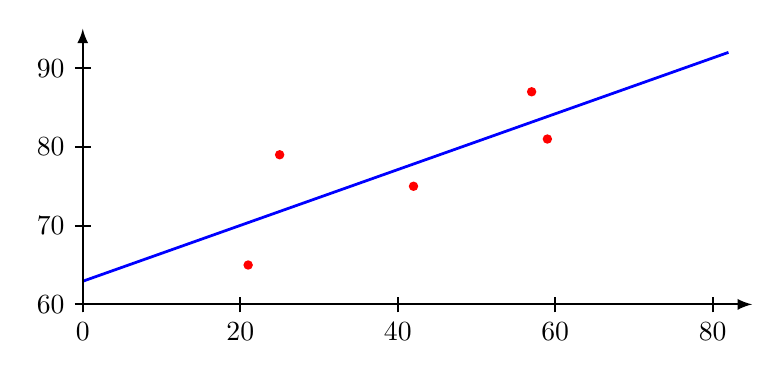
\begin{tikzpicture}[>=latex,thick,scale=0.1]
\def\punkt#1#2{
	\fill[color=red] (#1,#2) circle[radius=0.6];
}
\punkt{21}{65}
\punkt{25}{79}
\punkt{42}{75}
\punkt{57}{87}
\punkt{59}{81}
\draw[color=blue,line width=1pt]
	(0,62.938) -- (82,{82*0.35446+62.938});
\draw[->] (-1,60) -- (85,60);
\draw[->] ( 0,59) -- ( 0,95);
\def\strich#1{
	\draw (#1,59) -- (#1,61);
	\node at (#1,59) [below] {$#1$};
}
\strich{0}
\strich{20}
\strich{40}
\strich{60}
\strich{80}
\def\hstrich#1{
	\draw (-1,#1) -- (1,#1);
	\node at (-1,#1) [left] {$#1$};
}
\hstrich{60}
\hstrich{70}
\hstrich{80}
\hstrich{90}
\end{tikzpicture}
\end{center}
\end{teilaufgaben}
\end{loesung}

\begin{bewertung}
Methode der linearen Regression ({\bf L}) 1 Punkt,
Wert von $a$ ({\bf A}) 1 Punkt,
Wert von $b$ ({\bf B}) 1 Punkt,
Berechnung von $x$ ({\bf X}) 1 Punkt,
Wert von $r$ ({\bf R}) 1 Punkt,
Beurteilung mit Kriterium ``$r^2$ nahe bei 1'' ({\bf U}) 1 Punkt.
\end{bewertung}

% Quelle:  https://www.ques10.com/p/40606/example-of-linear-regression-1/

